\section{Módulo de Rastreamento}

	O Módulo de Rastreamento será responsável por rastrear os usuários no
	\textit{SmartSpace}, determinar a sua localização física em relação
	ao \textit{Kinect} e gerenciar suas identidades. Para realizar o rastreamento e
	localização dos usuários será utilizado a implementação existente na
	biblioteca \textit{OpenNI} (\textit{Open Natural Interaction}). Trata-se de um
	\textit{framework} que define \textit{APIs} para o desenvolvimento de
	aplicações de interação natural. Utilizando as imagens de
	profundidade, a detecção e o rastreamento é feito utilizando
	subtração de fundo~\ref{sec:deteccao-objeto} e os objetos detectados são
	representados por suas silhuetas~\ref{sec:representacao-objeto}.

	As imagens utilizadas para o rastreamento serão providas pelo \textit{Kinect} 
	e serão obtidas utilizando o método de Luz Estruturada descrito na
	Seção~\ref{sec:luz-estruturada}. Imagens de profundidade nada mais são que
	\textit{depth maps} (mapas de profundidade), em que cada pixel da imagem
	contém o valor estimado da distância em relação ao sensor. O \textit{Kinect}
	fornece esses dados a uma taxa de $\displaystyle 30 fps$ (\textit{frames} por
	segundo) com uma resolução $\displaystyle 320px$ x $\displaystyle 240px$.
	
	Utilizando os mapas de profundidade é possivel calcular as coodernadas
	$\displaystle (x,y,z)$, em relação ao sensor, de qualquer pixel da imagem.
	Dessa forma, qualquer usuário detectado na imagem tem implicita a sua
	localização. Sendo assim ao fixar a posição do \textit{Kinect} no
	ambiente, conseguiremos estimar a localização de qualquer usuário rastreado em
	tempo real.
	
	
	\begin{figure}[H]
		\begin{center}
			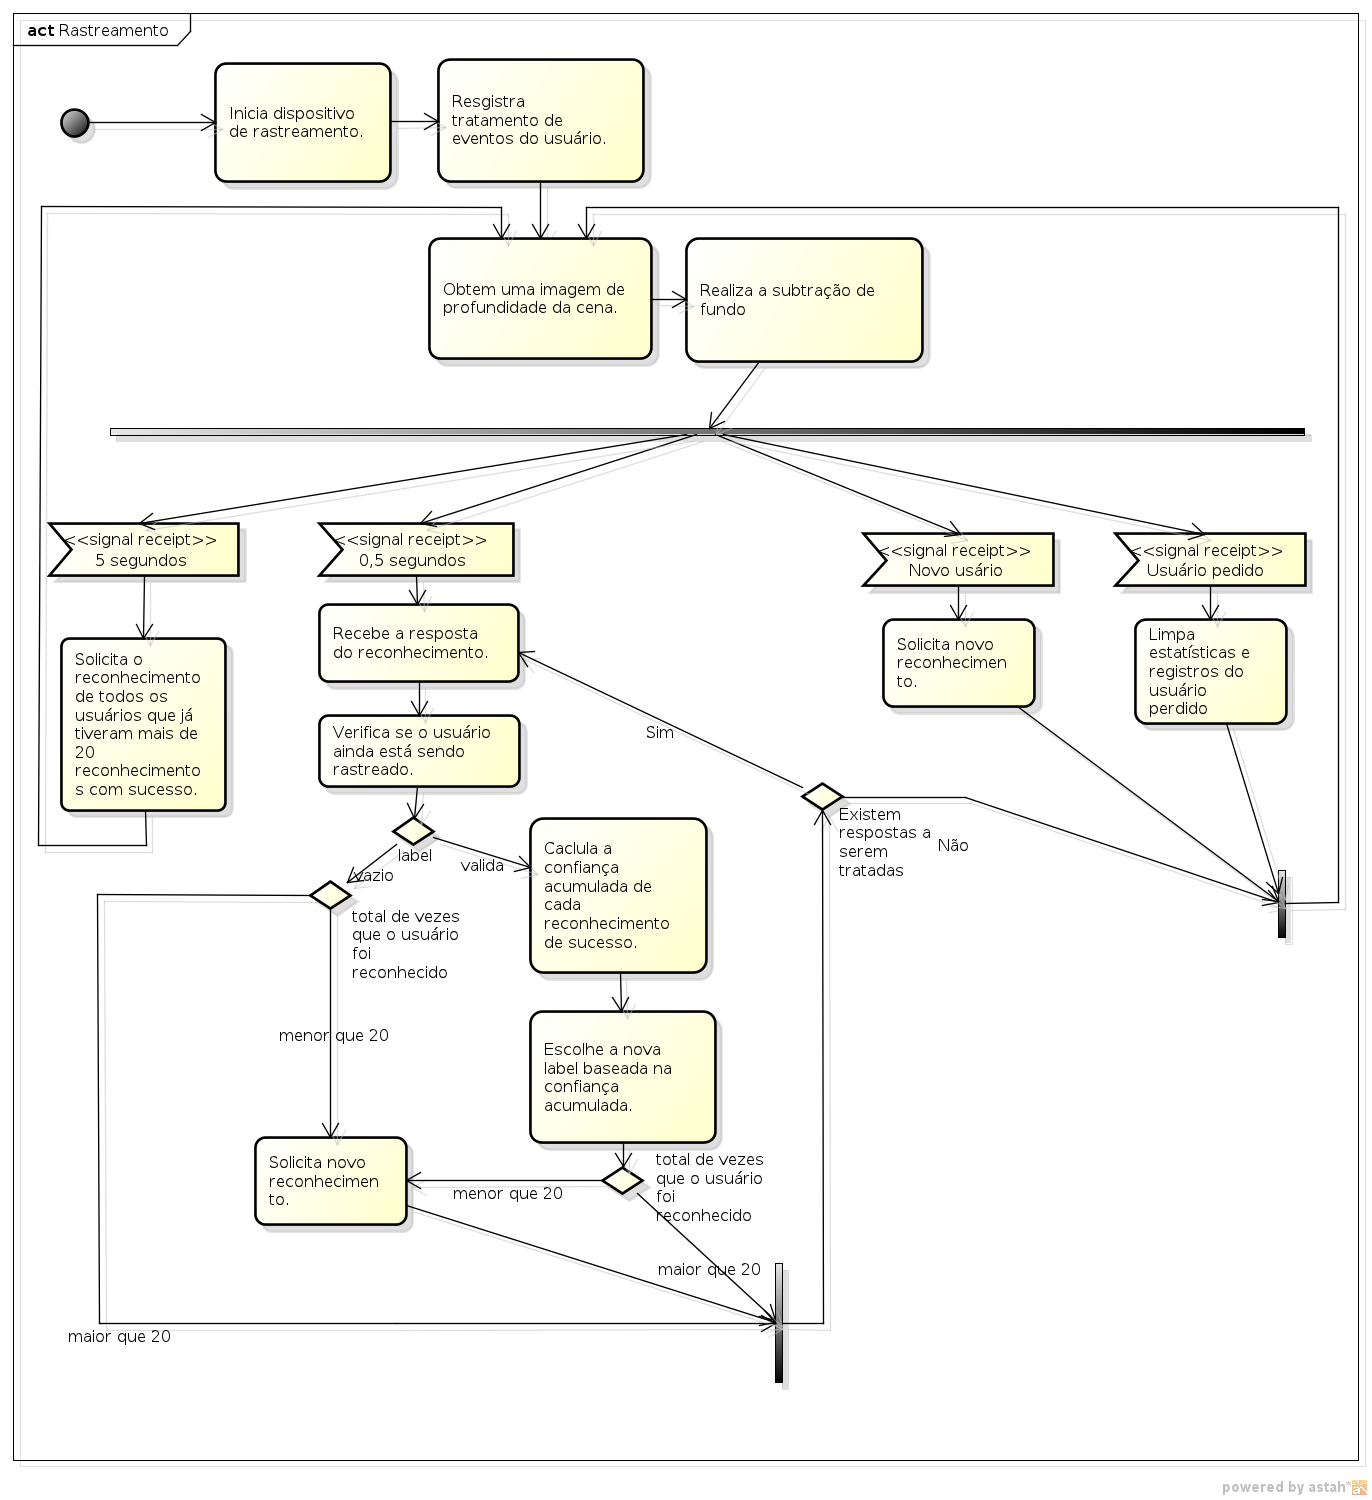
\includegraphics[scale=0.45]{figuras/4.ProblemaEProposta/Rastreamento.png}
		\end{center}
		\caption{Representação das etapas propostas para o rastreamento.}
		\label{fig:processo-rastreamento}
	\end{figure}
